\chapter{测试结果与分析}
\section{测试环境与版本}
实验开发与Windows验收于2026年11月9--10日进行，报告整理延续至11月11日。表\ref{tab:env}分别列出Windows原生环境与此前WSL环境。两者的编译器、文件系统和计时不同，不能将其数据混为同一次实验。

\begin{table}[H]\centering\caption{实际测试环境}\label{tab:env}
\small\begin{tabularx}{\linewidth}{lYY}\toprule
项目 & Windows原生 & 此前WSL2\\\midrule
操作系统 & Windows 11，10.0.26200 & Ubuntu 26.04 LTS，内核6.18.33.2-microsoft-standard-WSL2\\
CPU & \multicolumn{2}{l}{Intel Core i5-13500H，16个逻辑CPU}\\
编译器 & MSVC 19.44.35229 & GCC/g++ 15.2.0\\
工具集/SDK & 14.44.35207 / Windows SDK 10.0.26100.0 & Linux标准开发与线程库\\
构建 & CMake 4.4.4，C++11，Debug/Release & CMake 4.4.4，C++11，Release及检查配置\\
警告选项 & /W4 /utf-8，最终无编译警告 & -Wall -Wextra -Wpedantic\\
数据位置 & build/windows/run/配置；CTest在构建目录 & Linux用户缓存目录，非/mnt/c\\
编辑与调试 & VS Code 1.145.2，C/C++ 1.35.6，CMake Tools 1.24.42 & 命令行构建与测试\\\bottomrule
\end{tabularx}\end{table}

微软Build Tools安装包经Microsoft数字签名验证，在用户确认UAC后安装成功，复用现有CMake，不安装完整IDE。原生脚本通过\code{vswhere}发现MSVC，自动配置、增量构建并按真实退出码汇总结果。独立中文及空格路径也已从零编译并运行Project 3通过。

注释补充后的最终回归使用同一套十项验收，Debug和Release均通过。对全部17个C++文件剥离注释后逐项比较词法单元，与Windows兼容修正后的基线一致；没有更改算法、线程同步、文件格式或接口。最终提交及完整源码快照见第\ref{chap:source}章。

\section{测试数据与复现方法}
默认小输入为15个数，$M=4,B=3,k=3$，包含负数和重复值，能在少量输出内展示冻结、尾块、计划树及块回收。最终参考序列为
\begin{center}\small $[-1,0,1,2,2,3,3,4,5,6,7,8,9,10,12]$。\end{center}

自动测试有五组固定边界输入：空、单值、短逆序、重复负数和包含\code{INT32_MIN}、\code{INT32_MAX}的数组。随后使用\code{mt19937(20261109)}产生17、257、4099长度的值，取模101再减50，并派生升序、逆序版本，共14组。每组测试P1、P2及P3的$k=2,3,4$，合计70次。

再对固定15值组合$M=1,3,8$和$B=1,5,17$，三个项目共27次；40个种子0--39各产生一组长度小于100、值域$[-5,5]$的输入，随机选择$M=1\ldots9,B=1\ldots11,k=2\ldots7$，共120次。最后三个项目各检查50003个整数，总计$70+27+120+3=220$次。

Benchmark单独对$N=31,257,4099,50003$运行三个项目，固定$M=256,B=64,k=4$。每个规模重新初始化种子20261109，取模20001再减10000，各项目用相同输入。它的12次精确比较不包含在前述220次之中。\code{--size}演示与Benchmark均重新初始化随机生成器；测试套件末尾大输入使用套件内已经推进的生成器状态，二者不应被误认为逐项相同输入。

\begin{Verbatim}[fontsize=\small,numbers=none]
# 在仓库根目录的 PowerShell 中运行
.\验收.ps1 all -Configuration Debug
.\验收.ps1 all -Configuration Release
.\验收.ps1 project3 -K 2
.\验收.ps1 project3 -K 4 -Large
.\验收.ps1 benchmark -Configuration Release
\end{Verbatim}

同一运行目录不并发启动多个程序，防止固定测试文件名相互覆盖。不同平台采用独立构建目录；输出文件会重建，不能指向原始输入或其路径别名。报告所用CSV保留在\code{data/}，制图脚本只读取该快照，不把后续重跑时间自动替换进原表。

\section{正确性判据与实际结果}
\code{checkSort}独立复制输入并调用\code{std::sort}，从最终段分块读回，依次检查数量相等、非降序、逐项相等，再扫描每一个中间段检查有序。逐项相等同时覆盖重复次数；只检查有序性无法发现某些丢值问题。Release下断言使用抛异常的\code{require}，不会因\code{NDEBUG}失效。

\begin{table}[H]\centering\caption{最终Windows回归结果与此前WSL检查}\label{tab:regression}
\small\begin{tabularx}{\linewidth}{lYYY}\toprule
环境/配置 & 一键验收或检查 & CTest & CTest总时间\\\midrule
Windows Debug & 十项全部PASS，220次精确比较，12行Benchmark & 6/6 & 32.42 s\\
Windows Release & 十项全部PASS，220次精确比较，12行Benchmark & 6/6 & 26.85 s\\
此前WSL Release & 最终功能与Benchmark验证 & 6/6 & 10.29 s\\
此前WSL ASan+UBSan & 覆盖运行未见相关诊断 & 6/6 & 54.29 s\\
此前WSL TSan & 覆盖运行未见竞争诊断 & 6/6 & 14.02 s\\\bottomrule
\end{tabularx}\end{table}

表\ref{tab:regression}的时间是整个CTest套件时间，包含参考排序及所有检查，不是某次排序耗时。WSL的Sanitizer属于此前版本记录，不能写成Windows已经运行Sanitizer，也不是对所有输入的形式化证明。六项CTest为correctness、帮助和四种非法选项；非法参数测试以\code{WILL_FAIL}要求非零退出。

\begin{table}[H]\centering\caption{关键机制的目标、输入和判定}\label{tab:mechanisms}
\small\begin{tabularx}{\linewidth}{lYY}\toprule
机制 & 输入/操作 & 实际断言结果\\\midrule
文件与尾块 & 10个数、$B=3$，重开后读取 & 4次非空读、4次非空写，值完整\\
目录边界 & 容量2，已有两段后再beginRun & 拒绝；重名和无效段号亦拒绝\\
文件完整性 & 仅1字节裸文件、截断头部 & 拒绝，未被当作合法整数流\\
败者树 & 5叶候选4/3/6/8/1，冻结补0 & 冻结不抢先、重赛顺序正确、解冻后0可输出\\
最优树 & 段长1/2/3/100 & 普通212，最优115\\
共享池 & $k=3,B=1$，三路不同值域 & 一路占4块、块0回收后供路1\\
空路 & K路组内含空段、全空段 & 分别得到正确长度1和0\\
CLI错误 & B=0、M=-1、k=1、缺少size值 & 退出非零，CTest判定通过\\\bottomrule
\end{tabularx}\end{table}

\section{Windows真实运行截图}
以下图像直接采自VS Code运行真实Windows程序的窗口，LaTeX只裁去无关界面并按比例排版。截图来自Windows验收阶段，后续注释提交未改算法；最终回归记录见表\ref{tab:regression}。截图中Debug、trace、调试事件及暂停都可能影响计时，不能代替后文的Release性能数据。

\subsection{Week 3文件与缓冲验证}
图\ref{fig:shot-week3}显示Header=32、Directory=32、Data=416，A/B/C三段的实际偏移和长度，以及Search C=2、missing=$-1$。C通过容量2的输出缓冲写入5个数，包含尾块；重开后扫描值完整，符合模块设计。
\shot{windows-week3.png}{Week 3：真实文件创建、扫描、追加后的查询结果}{fig:shot-week3}{270bp 240bp 280bp 165bp}

\subsection{Project 1初始段与计划执行}
图\ref{fig:shot-p1}给出四个初始段、节点0--6的长度及孩子关系，再显示三次归并和最终15值。\code{theoretical_cost=30}与手算一致，最终完整比较PASS。段目录下标6对应M6，文件中仍保留初始与中间段。
\shot{windows-project1.png}{Project 1：分块内排、普通二叉计划及后序执行}{fig:shot-p1}{270bp 60bp 260bp 165bp}

\subsection{Project 2冻结、解冻与最优计划}
图\ref{fig:shot-p2}可看到候选2被标记frozen，随后\code{thaw -> run 2}；段长为7/7/1，普通代价29、最优23，执行R2+R0再与R1合并。最终精确结果相同，生成阶段6个同步阶段已经包含最后输出排空。
\shot{windows-project2-result.png}{Project 2：冻结状态、解冻、长段及最优二路计划}{fig:shot-p2}{270bp 12bp 240bp 180bp}

\subsection{Project 3动态池与K路归并}
图\ref{fig:shot-p3}展示每路队列中的物理块号、消费位置、loaded、last以及预取目标。\code{prefetch lane=1 block=2}证实原来属于路2的块回收后服务路1；末尾\code{produced=0}表示写出最后待写块。三路本例一次归并、一轮完成，最终段为K3。
\shot{windows-project3.png}{Project 3：动态预取、跨路块复用与最后阶段排空}{fig:shot-p3}{270bp 12bp 140bp 180bp}

\subsection{全部自动测试与实际断点}
图\ref{fig:shot-tests}同时显示机制测试、动态池测试与220次完整对照通过。九个具名配置均已实际启动；在\code{choosePrefetch}处F5命中断点，F10后观察到lane=0，并能查看调用堆栈。临时断点随后清除，继续运行得到PASS。另一次Ctrl+F5验证表明运行目录中的输入文件更新时间改变，仓库根旧文件未被改写。
\shot{windows-tests.png}{自动测试：局部机制、文件缓冲与220次精确比较通过}{fig:shot-tests}{270bp 180bp 110bp 180bp}

\section{性能指标与CSV结果}
\subsection{统计口径}
\code{reads/writes}是成功的非空数据块read/write调用，排除文件头、目录以及演示和验证扫描；不是物理磁盘I/O。\code{runs}指初始段数，\code{merges}指实际归并组数，\code{rounds}只对Project 3计数，Project 1/2的0不代表没有归并。\code{stages}累计置换选择与K路阶段，包括启动、等待和排空。

\code{ms}用\code{steady_clock}测量\code{sortFile}，从建立结果文件之前到归并完成，包括元数据、线程创建、join及刷新；不包括原始输入生成、参考排序和最终校验。Benchmark关闭trace。以下采用已保存的Windows Release单次数据，未作均值或冷缓存控制，后台负载和后续重跑可使时间变化。注释后回归的计数与该CSV一致，时间不要求相同。

\begin{table}[H]\centering\caption{Windows Release真实Benchmark，$M=256,B=64,k=4$}\label{tab:benchmark}
\scriptsize\setlength{\tabcolsep}{4pt}
\begin{tabular}{rrrrrrrrr}\toprule
项目 & $N$ & 段数 & 归并次数 & 轮数 & 块读 & 块写 & 阶段 & ms\\\midrule
1 & 31 & 1 & 0 & 0 & 1 & 1 & 0 & 3.7955 \\
2 & 31 & 1 & 0 & 0 & 1 & 1 & 2 & 4.74 \\
3 & 31 & 1 & 0 & 0 & 1 & 1 & 2 & 3.9383 \\
1 & 257 & 2 & 1 & 0 & 10 & 10 & 0 & 2.403 \\
2 & 257 & 1 & 0 & 0 & 5 & 5 & 6 & 3.0712 \\
3 & 257 & 1 & 0 & 0 & 5 & 5 & 6 & 2.8243 \\
1 & 4099 & 17 & 16 & 0 & 386 & 386 & 0 & 4.1211 \\
2 & 4099 & 9 & 8 & 0 & 273 & 278 & 66 & 14.3941 \\
3 & 4099 & 9 & 3 & 2 & 197 & 202 & 198 & 49.7333 \\
1 & 50003 & 196 & 195 & 0 & 6982 & 6982 & 0 & 57.579 \\
2 & 50003 & 99 & 98 & 0 & 6106 & 6152 & 783 & 160.114 \\
3 & 50003 & 99 & 34 & 4 & 3962 & 4008 & 3948 & 919.6 \\
\bottomrule

\end{tabular}\par\smallskip
\footnotesize 全部12行与\code{std::sort}精确比较均为PASS；数据源：\code{benchmark-windows.csv}。
\end{table}

\subsection{初始段、归并次数与轮数}
图\ref{fig:runs-chart}由同一CSV直接生成。$N=257$仅略超过$M=256$，普通分块生成2段，但该随机序列的置换选择形成1段，因此P2/P3无需再归并。$N=50003$时段数由196降为99，说明延长段实际减少了后续工作；不能据此推断逆序或所有分布都能减半。

\begin{figure}[H]\centering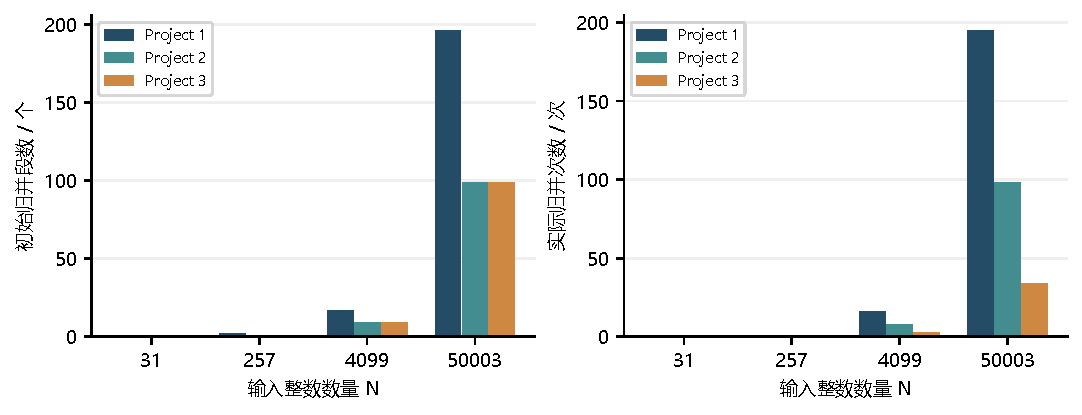
\includegraphics[width=\linewidth]{figures/runs-merges.pdf}\caption{Windows实测的初始段与归并次数；横轴按四个实验规模分类}\label{fig:runs-chart}\end{figure}

P2对99段二路合并98次，P3四路合并34次、4轮。只比较归并次数仍不充分，因为不同组处理的数据量不同，且部分单段直接带过。图\ref{fig:rounds-chart}单独给出P3轮数与阶段数，表明“轮数少”不等于“线程同步少”。
\begin{figure}[H]\centering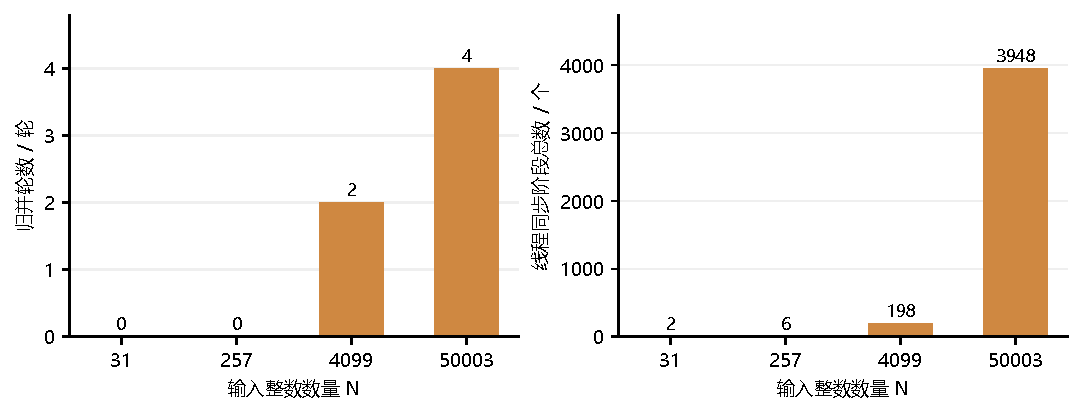
\includegraphics[width=\linewidth]{figures/rounds-stages.pdf}\caption{Project 3的归并轮数与三线程阶段总数，两个纵轴分别标注}\label{fig:rounds-chart}\end{figure}

默认15值下改变$k$也经过实际运行：$k=2$为2次归并、2轮，块读18、块写17；$k=3$与$k=4$都能把3个初始段一次合并，均为1轮、块读13、块写12。这里$k=4$仍分配8个输入块，但本组只有3路，说明配置容量与实际参与路数不同。

\subsection{数据块读写与实际时间}
图\ref{fig:io-time}比较最大实验规模的调用数，并展示四种规模的实际排序时间。$N=50003$时P1读写合计13964，P2为12258，P3为7970。P3相对P1减少约42.9\%的应用层数据块调用，但计时约为919.6 ms，高于P1的57.579 ms和P2的160.114 ms。

\begin{figure}[H]\centering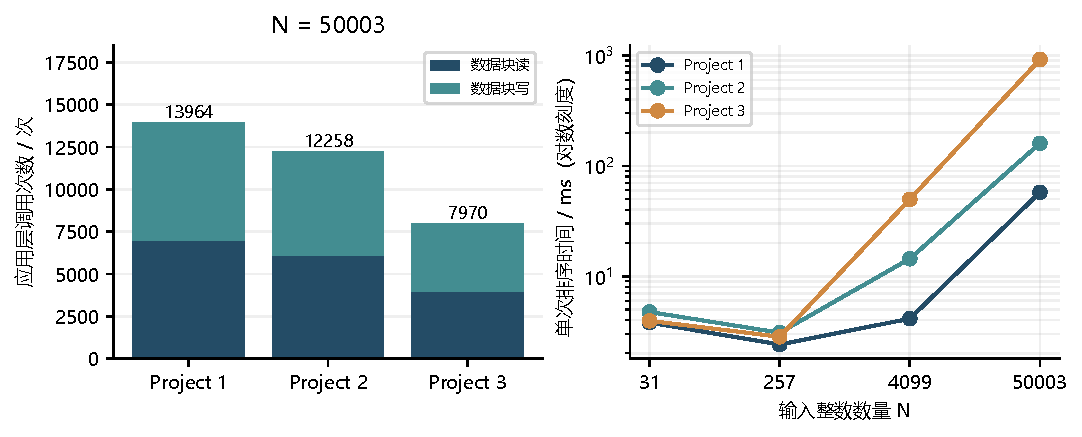
\includegraphics[width=\linewidth]{figures/io-time.pdf}\caption{Windows Release的数据块调用与单次耗时；时间纵轴使用对数刻度}\label{fig:io-time}\end{figure}

当前$B=64$仅为256字节，一个阶段产生的计算与I/O工作很少，而P3累计3948个同步阶段，每阶段新建并join三个线程。测试输入约200 KB，可被系统缓存，减少逻辑调用并不必然换来相应的物理磁盘节省。线程管理、调度和元数据操作可能占主导。这是对现象的合理解释，实验未单独测量每项开销，不能声称已精确分解各自占比。

\code{writes}不总等于\code{reads}：置换输出跨段时按段号分拆，K路缺头时可提前结束阶段并写出不足块的数据。小规模$N=31$时P2和P3执行同样的长段生成且无实际K路合并，单次时间仍不同，进一步说明不能把微小计时差异直接归因于算法结构。

\section{Windows与WSL的独立比较及解释边界}
\begin{table}[H]\centering\caption{$N=50003$时两环境的独立单次计时}\label{tab:platform-times}
\begin{tabular}{lrrr}\toprule 环境 & Project 1 / ms & Project 2 / ms & Project 3 / ms\\\midrule
Windows Release & 57.579 & 160.114 & 919.600\\
此前WSL Release & 21.4028 & 93.0083 & 379.418\\\bottomrule
\end{tabular}\end{table}

两份CSV除时间外，全部12行的段数、归并次数、轮数、块读写与阶段数逐项一致，支持算法行为在两种已测环境中一致。表\ref{tab:platform-times}不是操作系统性能排名：编译器、文件系统、缓存与运行时负载未被严格控制，不能把全部差异归于Windows或Linux本身。

同样$M,B,k$也不代表三项目总内存完全一致。P3持有更多输入块，置换选择有候选状态与段号标签，目录和计划随段数增长。最大输入50003个整数确实远超过候选容量256，能够触发多轮外排序流程，但尚未超过机器物理内存；不能将它描述为超大规模磁盘压力测试。

本实验支持的结论是：三种实现的正确性及课程机制在覆盖样本中得到验证；长段与K路归并减少了相关段数和应用层块调用；当前阶段线程实现并未在此测量条件下获得加速。更大的块、更多重复试验或线程复用可以作为后续研究，不能作为本报告已经完成的优化。
